\documentclass[12pt]{article}
\usepackage[utf8]{inputenc}
\usepackage{float}
\usepackage{amsmath}


\usepackage[hmargin=3cm,vmargin=6.0cm]{geometry}
%\topmargin=0cm
\topmargin=-2cm
\addtolength{\textheight}{6.5cm}
\addtolength{\textwidth}{2.0cm}
%\setlength{\leftmargin}{-5cm}
\setlength{\oddsidemargin}{0.0cm}
\setlength{\evensidemargin}{0.0cm}

%misc libraries goes here
\usepackage{tikz}
\usetikzlibrary{automata,positioning}

\begin{document}

\section*{Student Information } 
%Write your full name and id number between the colon and newline
%Put one empty space character after colon and before newline
Full Name : Kürşat Öztürk \\
Id Number :  2171874 \\

% Write your answers below the section tags
\section*{Answer 1}

\subsection*{a.}
Countable infinite. Set D = $\{$ -a/b:a,b$\in$ N and $a< b$ $\}$ Since N is countable, and we can map N to D, D is countably infinite.
\subsection*{b.}
Countable finite. Since L is finite, it is regular and so does $L^*$. Both L and $L^*$ is regular so $L^+$ is regular.(Recall that $L^+$ = $LL^*$).
So there are not any non-regular $L^+$.
Hence it is countably finite, because it is an empty set.
\subsection*{c.}
Uncoutably infinite.\\
There ara uncountably infinite language over the alphabet $\Sigma$. Regular ones, have the property being countable due to the Machines which accepts those languages that can be mapped to natural numbers; however, there is no alternative way to map non-regular languages since there does not exist any automota accepts those languages.So it is uncountably infinite.\\

\section*{Answer 2}

\begin{center}
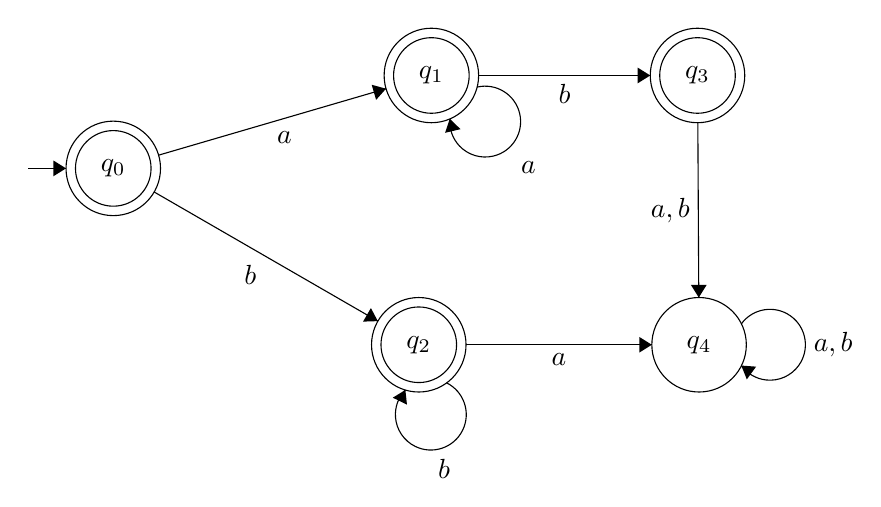
\begin{tikzpicture}[scale=0.2]
\tikzstyle{every node}+=[inner sep=0pt]
\draw [black] (15.6,-19.8) circle (3);
\draw (15.6,-19.8) node {$q_0$};
\draw [black] (15.6,-19.8) circle (2.4);
\draw [black] (35.8,-13.9) circle (3);
\draw (35.8,-13.9) node {$q_1$};
\draw [black] (35.8,-13.9) circle (2.4);
\draw [black] (52.7,-13.9) circle (3);
\draw (52.7,-13.9) node {$q_3$};
\draw [black] (52.7,-13.9) circle (2.4);
\draw [black] (35,-31) circle (3);
\draw (35,-31) node {$q_2$};
\draw [black] (35,-31) circle (2.4);
\draw [black] (52.8,-31) circle (3);
\draw (52.8,-31) node {$q_4$};
\draw [black] (18.48,-18.96) -- (32.92,-14.74);
\fill [black] (32.92,-14.74) -- (32.01,-14.49) -- (32.29,-15.45);
\draw (26.47,-17.4) node [below] {$a$};
\draw [black] (18.2,-21.3) -- (32.4,-29.5);
\fill [black] (32.4,-29.5) -- (31.96,-28.67) -- (31.46,-29.53);
\draw (24.3,-25.9) node [below] {$b$};
\draw [black] (52.72,-16.9) -- (52.78,-28);
\fill [black] (52.78,-28) -- (53.28,-27.2) -- (52.28,-27.2);
\draw (52.24,-22.45) node [left] {$a,b$};
\draw [black] (38,-31) -- (49.8,-31);
\fill [black] (49.8,-31) -- (49,-30.5) -- (49,-31.5);
\draw (43.9,-31.5) node [below] {$a$};
\draw [black] (38.8,-13.9) -- (49.7,-13.9);
\fill [black] (49.7,-13.9) -- (48.9,-13.4) -- (48.9,-14.4);
\draw (44.25,-14.4) node [below] {$b$};
\draw [black] (55.48,-29.677) arc (144:-144:2.25);
\draw (60.05,-31) node [right] {$a,b$};
\fill [black] (55.48,-32.32) -- (55.83,-33.2) -- (56.42,-32.39);
\draw [black] (38.695,-14.64) arc (103.39871:-184.60129:2.25);
\draw (41.47,-19.74) node [right] {$a$};
\fill [black] (36.97,-16.65) -- (36.67,-17.54) -- (37.65,-17.31);
\draw [black] (36.759,-33.416) arc (63.78241:-224.21759:2.25);
\draw (36.61,-38.25) node [below] {$b$};
\fill [black] (34.15,-33.87) -- (33.35,-34.36) -- (34.25,-34.8);
\draw [black] (10.2,-19.8) -- (12.6,-19.8);
\fill [black] (12.6,-19.8) -- (11.8,-19.3) -- (11.8,-20.3);
\end{tikzpicture}
\end{center}


\begin{center}
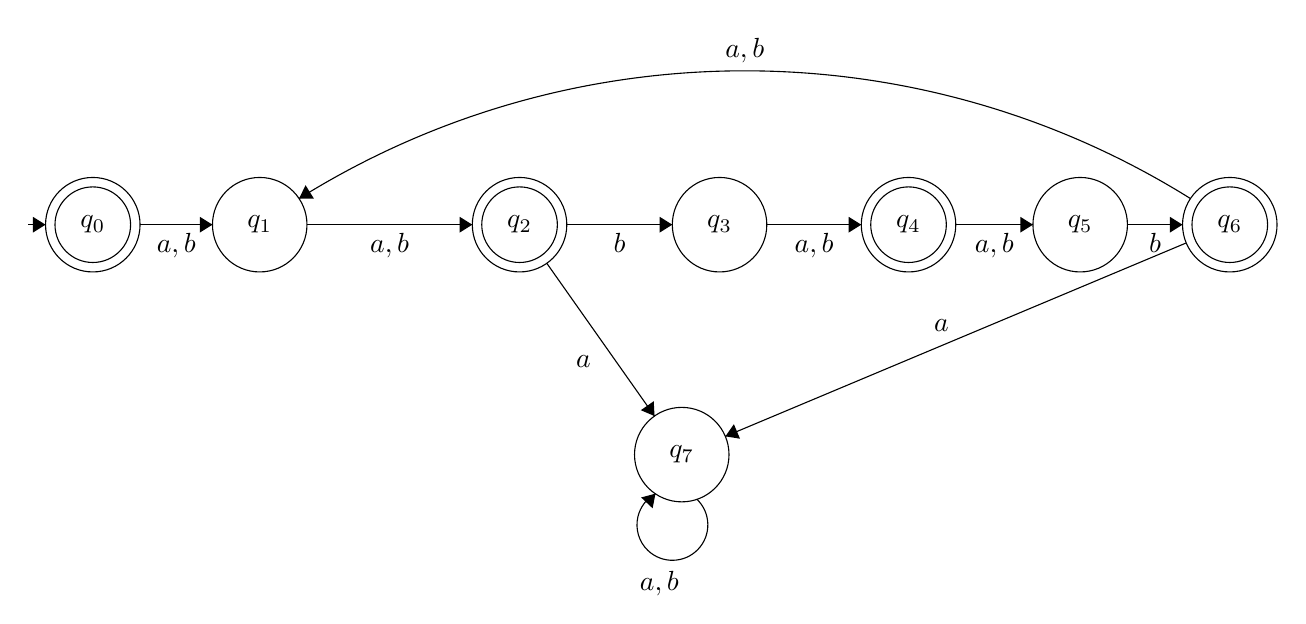
\begin{tikzpicture}[scale=0.2]
\tikzstyle{every node}+=[inner sep=0pt]
\draw [black] (4.7,-23.1) circle (3);
\draw (4.7,-23.1) node {$q_0$};
\draw [black] (4.7,-23.1) circle (2.4);
\draw [black] (15.3,-23.1) circle (3);
\draw (15.3,-23.1) node {$q_1$};
\draw [black] (31.8,-23.1) circle (3);
\draw (31.8,-23.1) node {$q_2$};
\draw [black] (31.8,-23.1) circle (2.4);
\draw [black] (44.5,-23.1) circle (3);
\draw (44.5,-23.1) node {$q_3$};
\draw [black] (56.5,-23.1) circle (3);
\draw (56.5,-23.1) node {$q_4$};
\draw [black] (56.5,-23.1) circle (2.4);
\draw [black] (67.4,-23.1) circle (3);
\draw (67.4,-23.1) node {$q_5$};
\draw [black] (76.9,-23.1) circle (3);
\draw (76.9,-23.1) node {$q_6$};
\draw [black] (76.9,-23.1) circle (2.4);
\draw [black] (42.1,-37.7) circle (3);
\draw (42.1,-37.7) node {$q_7$};
\draw [black] (7.7,-23.1) -- (12.3,-23.1);
\fill [black] (12.3,-23.1) -- (11.5,-22.6) -- (11.5,-23.6);
\draw (10,-23.6) node [below] {$a,b$};
\draw [black] (18.3,-23.1) -- (28.8,-23.1);
\fill [black] (28.8,-23.1) -- (28,-22.6) -- (28,-23.6);
\draw (23.55,-23.6) node [below] {$a,b$};
\draw [black] (34.8,-23.1) -- (41.5,-23.1);
\fill [black] (41.5,-23.1) -- (40.7,-22.6) -- (40.7,-23.6);
\draw (38.15,-23.6) node [below] {$b$};
\draw [black] (33.53,-25.55) -- (40.37,-35.25);
\fill [black] (40.37,-35.25) -- (40.32,-34.31) -- (39.5,-34.88);
\draw (36.36,-31.77) node [left] {$a$};
\draw [black] (47.5,-23.1) -- (53.5,-23.1);
\fill [black] (53.5,-23.1) -- (52.7,-22.6) -- (52.7,-23.6);
\draw (50.5,-23.6) node [below] {$a,b$};
\draw [black] (59.5,-23.1) -- (64.4,-23.1);
\fill [black] (64.4,-23.1) -- (63.6,-22.6) -- (63.6,-23.6);
\draw (61.95,-23.6) node [below] {$a,b$};
\draw [black] (70.4,-23.1) -- (73.9,-23.1);
\fill [black] (73.9,-23.1) -- (73.1,-22.6) -- (73.1,-23.6);
\draw (72.15,-23.6) node [below] {$b$};
\draw [black] (17.798,-21.44) arc (121.99229:58.00771:53.419);
\fill [black] (17.8,-21.44) -- (18.74,-21.44) -- (18.21,-20.59);
\draw (46.1,-12.83) node [above] {$a,b$};
\draw [black] (74.13,-24.26) -- (44.87,-36.54);
\fill [black] (44.87,-36.54) -- (45.8,-36.69) -- (45.41,-35.77);
\draw (58.59,-29.89) node [above] {$a$};
\draw [black] (43.057,-40.531) arc (46.40536:-241.59464:2.25);
\draw (40.68,-45.05) node [below] {$a,b$};
\fill [black] (40.43,-40.18) -- (39.52,-40.42) -- (40.25,-41.11);
\draw [black] (0.6,-23.1) -- (1.7,-23.1);
\fill [black] (1.7,-23.1) -- (0.9,-22.6) -- (0.9,-23.6);
\end{tikzpicture}
\end{center}





\begin{center}
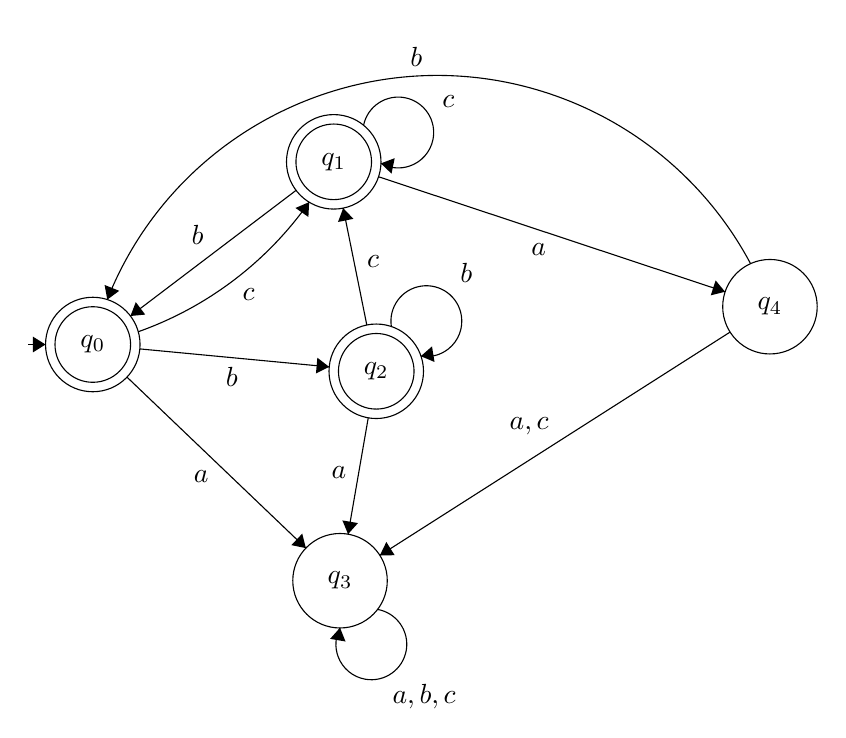
\begin{tikzpicture}[scale=0.2]
\tikzstyle{every node}+=[inner sep=0pt]
\draw [black] (4.7,-23.1) circle (3);
\draw (4.7,-23.1) node {$q_0$};
\draw [black] (4.7,-23.1) circle (2.4);
\draw [black] (20,-11.5) circle (3);
\draw (20,-11.5) node {$q_1$};
\draw [black] (20,-11.5) circle (2.4);
\draw [black] (22.7,-24.8) circle (3);
\draw (22.7,-24.8) node {$q_2$};
\draw [black] (22.7,-24.8) circle (2.4);
\draw [black] (20.4,-38.1) circle (3);
\draw (20.4,-38.1) node {$q_3$};
\draw [black] (47.7,-20.7) circle (3);
\draw (47.7,-20.7) node {$q_4$};
\draw [black] (0.6,-23.1) -- (1.7,-23.1);
\fill [black] (1.7,-23.1) -- (0.9,-22.6) -- (0.9,-23.6);
\draw [black] (18.44,-14.06) arc (-35.1851:-70.47828:22.466);
\fill [black] (18.44,-14.06) -- (17.57,-14.43) -- (18.39,-15);
\draw (14.6,-19.51) node [below] {$c$};
\draw [black] (17.61,-13.31) -- (7.09,-21.29);
\fill [black] (7.09,-21.29) -- (8.03,-21.2) -- (7.43,-20.41);
\draw (11.35,-16.8) node [above] {$b$};
\draw [black] (7.69,-23.38) -- (19.71,-24.52);
\fill [black] (19.71,-24.52) -- (18.96,-23.94) -- (18.87,-24.94);
\draw (13.53,-24.53) node [below] {$b$};
\draw [black] (23.66,-21.97) arc (189:-99:2.25);
\draw (28,-18.55) node [right] {$b$};
\fill [black] (25.53,-23.84) -- (26.4,-24.21) -- (26.24,-23.22);
\draw [black] (22.77,-39.92) arc (80.21401:-207.78599:2.25);
\draw (25.74,-44.67) node [below] {$a,b,c$};
\fill [black] (20.4,-41.09) -- (19.77,-41.79) -- (20.75,-41.96);
\draw [black] (22.19,-27.76) -- (20.91,-35.14);
\fill [black] (20.91,-35.14) -- (21.54,-34.44) -- (20.55,-34.27);
\draw (20.83,-31.21) node [left] {$a$};
\draw [black] (6.87,-25.17) -- (18.23,-36.03);
\fill [black] (18.23,-36.03) -- (18,-35.11) -- (17.31,-35.84);
\draw (11.59,-31.08) node [below] {$a$};
\draw [black] (22.1,-21.86) -- (20.6,-14.44);
\fill [black] (20.6,-14.44) -- (20.27,-15.32) -- (21.25,-15.12);
\draw (22.09,-17.83) node [right] {$c$};
\draw [black] (22.85,-12.45) -- (44.85,-19.75);
\fill [black] (44.85,-19.75) -- (44.25,-19.03) -- (43.94,-19.98);
\draw (33.01,-16.63) node [below] {$a$};
\draw [black] (45.17,-22.31) -- (22.93,-36.49);
\fill [black] (22.93,-36.49) -- (23.87,-36.48) -- (23.34,-35.64);
\draw (32.41,-28.9) node [above] {$a,c$};
\draw [black] (5.618,-20.246) arc (158.35541:28.03377:22.543);
\fill [black] (5.62,-20.25) -- (6.38,-19.69) -- (5.45,-19.32);
\draw (25.25,-5.5) node [above] {$b$};
\draw [black] (21.892,-9.187) arc (168.44395:-119.55605:2.25);
\draw (26.87,-7.69) node [right] {$c$};
\fill [black] (22.99,-11.6) -- (23.67,-12.25) -- (23.87,-11.27);
\end{tikzpicture}
\end{center}



\section*{Answer 3}


\subsection*{a.}

$w_1$ = abbb is not in L(N). $w_1$ ends with "b" and to reach final states(in this case, only $q_5$), an "a" must be read from input. In this case, input will end in an not-accepting state in all possible computings.Hence, $w_1$ is not in L(N).\\
\subsection*{b.}
 $(q_0,a,q_1),(q_1,e,q_3),(q_3,b,q_3),(q_3,a,q_1),(q_1,e,q_3),(q_3,b,q_3),(q_3,a,q_5)$\\
Input stop when it is in final state, so it is in L(N) \\



\section*{Answer 4}

\subsection*{a.}
$M_G = (K_G,\Sigma,\Delta,s_G,F_G)$\\
$K_G = \{q_1,q_2,q_3,q_4,q_5,q_6\}$\\
$\Sigma = \{a,b\}$\\
$s_G = q_5$ $F_G = \{ q_6\}$\\
$\Delta_G = \{(q_1,b,q_2),$\\

$(q_2,a,q_3),(q_2,e,q_4),$\\

$(q,3,a,q_1),(q_3,b,q_2),(q_3,b,q_3),(q_3,b,q_4),(q_3,e,q_6),$\\

$(q_4,b,q_2),(q_4,a,q_4),(q_4,e,q_6),$\\

$(q_5,e,q_1)\}$\\

\begin{center}
\begin{tikzpicture}[scale=0.2]
\tikzstyle{every node}+=[inner sep=0pt]
\draw [black] (4.3,-18.1) circle (3);
\draw (4.3,-18.1) node {$q_5$};
\draw [black] (19.2,-18.1) circle (3);
\draw (19.2,-18.1) node {$q_1$};
\draw [black] (35.7,-18.1) circle (3);
\draw (35.7,-18.1) node {$q_2$};
\draw [black] (58.6,-18.1) circle (3);
\draw (58.6,-18.1) node {$q_3$};
\draw [black] (34.5,-35.4) circle (3);
\draw (34.5,-35.4) node {$q_4$};
\draw [black] (58.6,-35.4) circle (3);
\draw (58.6,-35.4) node {$q_6$};
\draw [black] (7.3,-18.1) -- (16.2,-18.1);
\fill [black] (16.2,-18.1) -- (15.4,-17.6) -- (15.4,-18.6);
\draw (11.75,-18.6) node [below] {$e$};
\draw [black] (22.2,-18.1) -- (32.7,-18.1);
\fill [black] (32.7,-18.1) -- (31.9,-17.6) -- (31.9,-18.6);
\draw (27.45,-18.6) node [below] {$b$};
\draw [black] (37.782,-15.948) arc (130.04011:49.95989:14.561);
\fill [black] (56.52,-15.95) -- (56.23,-15.05) -- (55.58,-15.82);
\draw (47.15,-12.03) node [above] {$a$};
\draw [black] (60.096,-15.513) arc (177.69007:-110.30993:2.25);
\draw (64.83,-13.02) node [right] {$b$};
\fill [black] (61.56,-17.71) -- (62.34,-18.25) -- (62.38,-17.25);
\draw [black] (55.6,-18.1) -- (38.7,-18.1);
\fill [black] (38.7,-18.1) -- (39.5,-18.6) -- (39.5,-17.6);
\draw (47.15,-17.6) node [above] {$b$};
\draw [black] (33.411,-32.609) arc (-163.68657:-204.24927:17.198);
\fill [black] (33.41,-32.61) -- (33.67,-31.7) -- (32.71,-31.98);
\draw (32.16,-26.55) node [left] {$e$};
\draw [black] (34.71,-32.41) -- (35.49,-21.09);
\fill [black] (35.49,-21.09) -- (34.94,-21.86) -- (35.94,-21.93);
\draw (35.7,-26.79) node [right] {$b$};
\draw [black] (56.16,-19.85) -- (36.94,-33.65);
\fill [black] (36.94,-33.65) -- (37.88,-33.59) -- (37.3,-32.78);
\draw (45.55,-26.25) node [above] {$b$};
\draw [black] (37.5,-35.4) -- (55.6,-35.4);
\fill [black] (55.6,-35.4) -- (54.8,-34.9) -- (54.8,-35.9);
\draw (46.55,-35.9) node [below] {$e$};
\draw [black] (58.6,-21.1) -- (58.6,-32.4);
\fill [black] (58.6,-32.4) -- (59.1,-31.6) -- (58.1,-31.6);
\draw (58.1,-26.75) node [left] {$e$};
\draw [black] (20.477,-15.388) arc (150.71042:29.28958:21.123);
\fill [black] (20.48,-15.39) -- (21.3,-14.94) -- (20.43,-14.45);
\draw (38.9,-4.1) node [above] {$a$};
\draw [black] (32.503,-37.623) arc (-14.19859:-302.19859:2.25);
\draw (27.49,-38.79) node [left] {$a$};
\fill [black] (31.52,-35.17) -- (30.87,-34.49) -- (30.62,-35.46);
\draw [black] (0.7,-18.1) -- (1.3,-18.1);
\fill [black] (1.3,-18.1) -- (0.5,-17.6) -- (0.5,-18.6);
\end{tikzpicture}
\end{center}


\subsection*{b.}

\begin{center}
\begin{tikzpicture}[scale=0.2]
\tikzstyle{every node}+=[inner sep=0pt]
\draw [black] (4.3,-18.1) circle (3);
\draw (4.3,-18.1) node {$q_5$};
\draw [black] (19.2,-18.1) circle (3);
\draw (19.2,-18.1) node {$q_1$};
\draw [black] (35.7,-18.1) circle (3);
\draw (35.7,-18.1) node {$q_2$};
\draw [black] (58.6,-18.1) circle (3);
\draw (58.6,-18.1) node {$q_3$};
\draw [black] (58.6,-35.4) circle (3);
\draw (58.6,-35.4) node {$q_6$};
\draw [black](58.6,-35.4) circle (2.4);
\draw [black] (7.3,-18.1) -- (16.2,-18.1);
\fill [black] (16.2,-18.1) -- (15.4,-17.6) -- (15.4,-18.6);
\draw (11.75,-18.6) node [below] {$e$};
\draw [black] (22.2,-18.1) -- (32.7,-18.1);
\fill [black] (32.7,-18.1) -- (31.9,-17.6) -- (31.9,-18.6);
\draw (27.45,-18.6) node [below] {$b$};
\draw [black] (37.782,-15.948) arc (130.04011:49.95989:14.561);
\fill [black] (56.52,-15.95) -- (56.23,-15.05) -- (55.58,-15.82);
\draw (47.15,-12.03) node [above] {$a$};
\draw [black] (60.096,-15.513) arc (177.69007:-110.30993:2.25);
\draw (64.83,-13.02) node [right] {$b$};
\fill [black] (61.56,-17.71) -- (62.34,-18.25) -- (62.38,-17.25);
\draw [black] (55.6,-18.1) -- (38.7,-18.1);
\fill [black] (38.7,-18.1) -- (39.5,-18.6) -- (39.5,-17.6);
\draw (47.15,-17.6) node [above] {$b$};
\draw [black] (58.6,-21.1) -- (58.6,-32.4);
\fill [black] (58.6,-32.4) -- (59.1,-31.6) -- (58.1,-31.6);
\draw (58.1,-26.75) node [left] {$ba^*$};
\draw [black] (20.477,-15.388) arc (150.71042:29.28958:21.123);
\fill [black] (20.48,-15.39) -- (21.3,-14.94) -- (20.43,-14.45);
\draw (38.9,-4.1) node [above] {$a$};
\draw [black] (0.7,-18.1) -- (1.3,-18.1);
\fill [black] (1.3,-18.1) -- (0.5,-17.6) -- (0.5,-18.6);
\draw [black] (38.09,-19.91) -- (56.21,-33.59);
\fill [black] (56.21,-33.59) -- (55.87,-32.71) -- (55.27,-33.51);
\draw (45.7,-27.25) node [below] {$a^*$};
\draw [black] (34.377,-15.42) arc (234:-54:2.25);
\draw (35.7,-10.85) node [above] {$a^*bUab^*ba^*b$};
\fill [black] (37.02,-15.42) -- (37.9,-15.07) -- (37.09,-14.48);
\end{tikzpicture}
\end{center}


\begin{center}
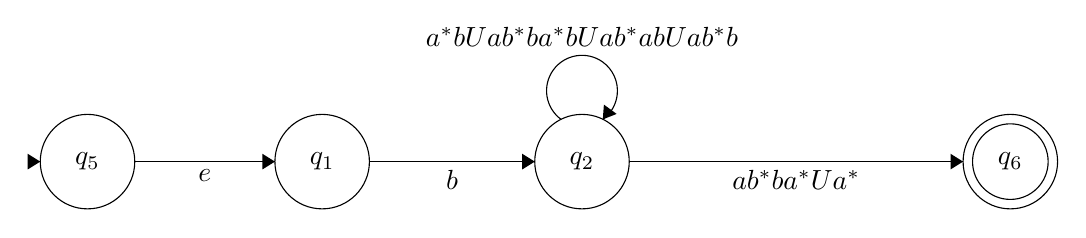
\begin{tikzpicture}[scale=0.2]
\tikzstyle{every node}+=[inner sep=0pt]
\draw [black] (4.3,-18.1) circle (3);
\draw (4.3,-18.1) node {$q_5$};
\draw [black] (19.2,-18.1) circle (3);
\draw (19.2,-18.1) node {$q_1$};
\draw [black] (35.7,-18.1) circle (3);
\draw (35.7,-18.1) node {$q_2$};
\draw [black] (62.9,-18.1) circle (3);
\draw (62.9,-18.1) node {$q_6$};
\draw [black] (62.9,-18.1) circle (2.4);
\draw [black] (7.3,-18.1) -- (16.2,-18.1);
\fill [black] (16.2,-18.1) -- (15.4,-17.6) -- (15.4,-18.6);
\draw (11.75,-18.6) node [below] {$e$};
\draw [black] (22.2,-18.1) -- (32.7,-18.1);
\fill [black] (32.7,-18.1) -- (31.9,-17.6) -- (31.9,-18.6);
\draw (27.45,-18.6) node [below] {$b$};
\draw [black] (0.7,-18.1) -- (1.3,-18.1);
\fill [black] (1.3,-18.1) -- (0.5,-17.6) -- (0.5,-18.6);
\draw [black] (38.7,-18.1) -- (59.9,-18.1);
\fill [black] (59.9,-18.1) -- (59.1,-17.6) -- (59.1,-18.6);
\draw (49.3,-18.6) node [below] {$ab^*ba^*Ua^*$};
\draw [black] (34.377,-15.42) arc (234:-54:2.25);
\draw (35.7,-10.85) node [above] {$a^*bUab^*ba^*bUab^*abUab^*b$};
\fill [black] (37.02,-15.42) -- (37.9,-15.07) -- (37.09,-14.48);
\end{tikzpicture}
\end{center}


\begin{center}
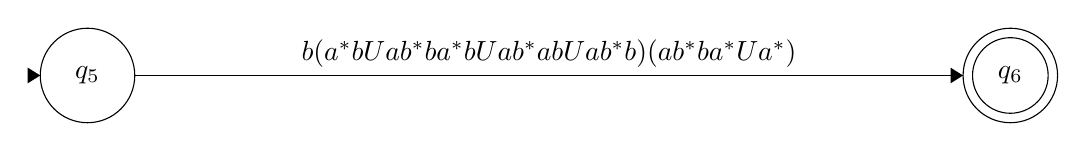
\begin{tikzpicture}[scale=0.2]
\tikzstyle{every node}+=[inner sep=0pt]
\draw [black] (4.3,-18.1) circle (3);
\draw (4.3,-18.1) node {$q_5$};
\draw [black] (62.9,-18.1) circle (3);
\draw (62.9,-18.1) node {$q_6$};
\draw [black] (62.9,-18.1) circle (2.4);
\draw [black] (0.7,-18.1) -- (1.3,-18.1);
\fill [black] (1.3,-18.1) -- (0.5,-17.6) -- (0.5,-18.6);
\draw [black] (7.3,-18.1) -- (59.9,-18.1);
\fill [black] (59.9,-18.1) -- (59.1,-17.6) -- (59.1,-18.6);
\draw (33.6,-17.6) node [above] {$b(a^*bUab^*ba^*bUab^*abUab^*b)(ab^*ba^*Ua^*)$};
\end{tikzpicture}
\end{center}




\section*{Answer 5}

\begin{center}
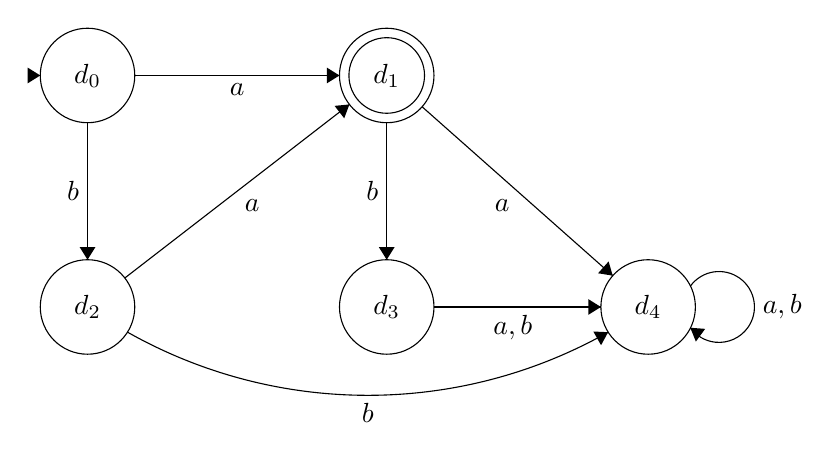
\begin{tikzpicture}[scale=0.2]
\tikzstyle{every node}+=[inner sep=0pt]
\draw [black] (9.4,-13.9) circle (3);
\draw (9.4,-13.9) node {$d_0$};
\draw [black] (28.4,-13.9) circle (3);
\draw (28.4,-13.9) node {$d_1$};
\draw [black] (28.4,-13.9) circle (2.4);
\draw [black] (9.4,-28.6) circle (3);
\draw (9.4,-28.6) node {$d_2$};
\draw [black] (28.4,-28.6) circle (3);
\draw (28.4,-28.6) node {$d_3$};
\draw [black] (45,-28.6) circle (3);
\draw (45,-28.6) node {$d_4$};
\draw [black] (9.4,-16.9) -- (9.4,-25.6);
\fill [black] (9.4,-25.6) -- (9.9,-24.8) -- (8.9,-24.8);
\draw (8.9,-21.25) node [left] {$b$};
\draw [black] (12.4,-13.9) -- (25.4,-13.9);
\fill [black] (25.4,-13.9) -- (24.6,-13.4) -- (24.6,-14.4);
\draw (18.9,-14.4) node [below] {$a$};
\draw [black] (11.77,-26.76) -- (26.03,-15.74);
\fill [black] (26.03,-15.74) -- (25.09,-15.83) -- (25.7,-16.62);
\draw (19.85,-21.75) node [below] {$a$};
\draw [black] (28.4,-16.9) -- (28.4,-25.6);
\fill [black] (28.4,-25.6) -- (28.9,-24.8) -- (27.9,-24.8);
\draw (27.9,-21.25) node [left] {$b$};
\draw [black] (30.65,-15.89) -- (42.75,-26.61);
\fill [black] (42.75,-26.61) -- (42.49,-25.71) -- (41.82,-26.46);
\draw (35.74,-21.74) node [below] {$a$};
\draw [black] (31.4,-28.6) -- (42,-28.6);
\fill [black] (42,-28.6) -- (41.2,-28.1) -- (41.2,-29.1);
\draw (36.7,-29.1) node [below] {$a,b\mbox{ }$};
\draw [black] (42.463,-30.199) arc (-60.54503:-119.45497:31.039);
\fill [black] (42.46,-30.2) -- (41.52,-30.16) -- (42.01,-31.03);
\draw (27.2,-34.71) node [below] {$b$};
\draw [black] (6,-13.9) -- (6.4,-13.9);
\fill [black] (6.4,-13.9) -- (5.6,-13.4) -- (5.6,-14.4);
\draw [black] (47.68,-27.277) arc (144:-144:2.25);
\draw (52.25,-28.6) node [right] {$a,b$};
\fill [black] (47.68,-29.92) -- (48.03,-30.8) -- (48.62,-29.99);
\end{tikzpicture}
\end{center}


.\\\\
where $d_0=\{q_0,q_1,q_2\}$\\
$d_1=\{q_1,q_3\}$\\
$d_2= \{q_2\}$\\
$d_3=\{q_1\}$\\
$d_4 =\{\}$\\

\begin{center}
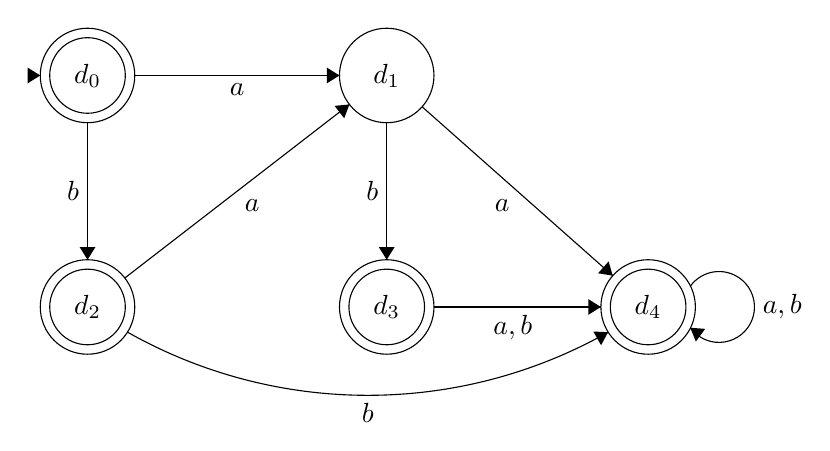
\begin{tikzpicture}[scale=0.2]
\tikzstyle{every node}+=[inner sep=0pt]
\draw [black] (9.4,-13.9) circle (3);
\draw (9.4,-13.9) node {$d_0$};
\draw [black] (9.4,-13.9) circle (2.4);
\draw [black] (28.4,-13.9) circle (3);
\draw (28.4,-13.9) node {$d_1$};
\draw [black] (9.4,-28.6) circle (3);
\draw (9.4,-28.6) node {$d_2$};
\draw [black] (9.4,-28.6) circle (2.4);
\draw [black] (28.4,-28.6) circle (3);
\draw (28.4,-28.6) node {$d_3$};
\draw [black] (28.4,-28.6) circle (2.4);
\draw [black] (45,-28.6) circle (3);
\draw (45,-28.6) node {$d_4$};
\draw [black] (45,-28.6) circle (2.4);
\draw [black] (9.4,-16.9) -- (9.4,-25.6);
\fill [black] (9.4,-25.6) -- (9.9,-24.8) -- (8.9,-24.8);
\draw (8.9,-21.25) node [left] {$b$};
\draw [black] (12.4,-13.9) -- (25.4,-13.9);
\fill [black] (25.4,-13.9) -- (24.6,-13.4) -- (24.6,-14.4);
\draw (18.9,-14.4) node [below] {$a$};
\draw [black] (11.77,-26.76) -- (26.03,-15.74);
\fill [black] (26.03,-15.74) -- (25.09,-15.83) -- (25.7,-16.62);
\draw (19.85,-21.75) node [below] {$a$};
\draw [black] (28.4,-16.9) -- (28.4,-25.6);
\fill [black] (28.4,-25.6) -- (28.9,-24.8) -- (27.9,-24.8);
\draw (27.9,-21.25) node [left] {$b$};
\draw [black] (30.65,-15.89) -- (42.75,-26.61);
\fill [black] (42.75,-26.61) -- (42.49,-25.71) -- (41.82,-26.46);
\draw (35.74,-21.74) node [below] {$a$};
\draw [black] (31.4,-28.6) -- (42,-28.6);
\fill [black] (42,-28.6) -- (41.2,-28.1) -- (41.2,-29.1);
\draw (36.7,-29.1) node [below] {$a,b\mbox{ }$};
\draw [black] (42.463,-30.199) arc (-60.54503:-119.45497:31.039);
\fill [black] (42.46,-30.2) -- (41.52,-30.16) -- (42.01,-31.03);
\draw (27.2,-34.71) node [below] {$b$};
\draw [black] (6,-13.9) -- (6.4,-13.9);
\fill [black] (6.4,-13.9) -- (5.6,-13.4) -- (5.6,-14.4);
\draw [black] (47.68,-27.277) arc (144:-144:2.25);
\draw (52.25,-28.6) node [right] {$a,b$};
\fill [black] (47.68,-29.92) -- (48.03,-30.8) -- (48.62,-29.99);
\end{tikzpicture}
\end{center}
regular expression for above language: \\
$eUb U ab U bab U baa(aUb)^* U bab(aUb)(aUb)^*Uab(aUb)(aUb)^*Uaa(aUb)^*$\\


\section*{Answer 6}

$M_1 = (K_1,\Sigma_1,\Delta_1,s_1,F_1)$ \\
$M_2 = (K_2,\Sigma_2,\Delta_2,s_2,F_2)$ \\

$M = (K,\Sigma,\Delta,s,F)$ \\

$ K = K_1 x K_2$ \\

$\Sigma  =\Sigma_1 \bigcup \Sigma_2$

$\Delta = \{((q_1,q_2),w,(q_1',q_2'))|w \in \Sigma, (q_1,w,q_1') \in \Delta_1, (q_2,w,q_2') \in \Delta_2\}$\\
$s = (s_1,s_2)$\\
$F = \{(q_1,q_2)|q_1 \in F_1,q_2 \in K_2-F_2\}$\\

1)\\

$L(M) \subseteq L(M_1) - L(M_2)$ \\

Assume $x\in L(M)$, states $\rightarrow (p,q)$\\

$M_1$ accepts x, since p is accepting state for $M_1$\\
$M_2$ doesn't accept x, since q is not-accepting state for $M_2$\\
so it holds. \\

$L(M_1)-L(M_2) \subseteq L(M)$\\


Assume $x\in L(M_1)-L(M_2)$, states $\rightarrow$(p,q)\\

$M_1$ accepts x, since p is accepting state for $M_1$\\
$M_2$ doesn't accept x, since q is not-accepting state for $M_2$\\
(p,q) is accepted by L(M) by construction \\
so it holds. \\

Since both are true $L(M) = L(M_1)-L(M_2)$ \\

\section*{Answer 7}

 p = pumping length\\

$ = a^{p^2}$ $s\in L$ \\

$|s|$ = $p^2 \geq p$\\, so the  Pumping Lemma will hold. So, S can be split into 3 part as s = xyz satisfying \\
1) $xy^{i}z \in L $ for each $i\geq0$\\
2) $|y|>0$\\
3) $|xy|\leq p$\\

x = $a^k$\\
y = $a^l$\\
z = $a^{p^2-k-l}$, where $k+l \leq p $ and $l \geq 0$ \\
when choose i = 2 to get $xy^2z$ \\
$a^k a^{2l} a^{p^2-k-l} = a^{p^2+l}$ \\
$l>0 \rightarrow p^2 + l > p$ \\
$ l \leq p \rightarrow p^2 + l \leq p^2 + p < p^2 + 2p + 1 = (p+1)^2$ \\

$p^2 < p^2 + l < (p+1)^2$ \\
So $p^2 + l$ cannot be a square of an integer.\\


\end{document}

​

